\documentclass[12pt,a4paper]{article}

\usepackage{amsfonts,amssymb,amsmath,amsthm}
\usepackage{stmaryrd} %for special brackets
\usepackage{lipsum}
\usepackage{graphicx}
\graphicspath{img}
\usepackage[hidelinks]{hyperref}
\usepackage{array}
\usepackage{bm} %for bold in math equations
\usepackage{float} %to force the position of some figures
\usepackage{biblatex}
\usepackage{geometry}
\usepackage{todonotes}


\addbibresource{_report.bib}
\geometry{left=2.54cm,right=2.54cm}


\title{Internship Report}
\author{Lucas SALAND}
\date{\today}

\begin{document}
\maketitle
\newpage
\tableofcontents
\newpage

\section*{Introduction}
This M1 internship was carried out at CRIStAL in the SIGMA team under the supervision of Patrick Bas. The internship lasted for three months during which we worked on a challenge from the AID on the detection of images generated by AI.\\
CRIStAL is a laboratory which research focus on computer science, signal and automatic control. It is under the supervision of the University of Lille, CNRS and Centrale Lille. The laboratory is divided in 34 research teams grouped in 9 Thematic Groups. SIGMA team is part of DatInG : Data Intelligence Group. SIGMA is a team of 15 permanent staff which focuses on machine learning, statistics and signal processing. Some of the research topics are Monte-Carlo methods, signal processing with tensorial approaches and information security.
\todo[inline]{develop on the team environment (saw a phd defense, sigma day)}

The Agence de l'innovation et de défense (AID) launched a challenge on detecting modified or generated images. This challenge aimed at detecting three types of images :
\begin{itemize}
    \item fully AI-generated images;
    \item images partially modified by AI;
    \item images partially modified with more usual image processing tools such as photoshop.
\end{itemize}
This challenge was divided in two tasks : A and B. Task A focused on images fully generated by AI. AId first provided a sample of images to give an idea of what would be the testing data would be. Images provided were compressed with JPEG. Our team identified 3 quality factors for compression: 40, 65 and 90. AID then provided 10000 images on the last day of the challenge. The goal was to identify which images were real and which one were generated. On top of this, we could provide which generator was used to generate images. Task A could be treated as binary classification problem with the two classes being real and generated images. It could also be treated as a multi-class classification problem where the classes would be the real images and all the generator used. The main difficulty was that the generators used were kept secret until the last day of the challenge.\\
Task B focused on the detection of partially modified images. The objectives were :
\begin{itemize}
    \item detecting real images and modified images;
    \item identifying the tool used for modification;
    \item localisation of modification on images.
\end{itemize}

I worked on the challenge in a team with 3 other interns and 5 permanent staff from SIGMA. During the internship, I worked on task A.


\section{AI-generated images detection}
\subsection{AI image generation}
We should now go over an overview of image generation with AI. In recent years, the quality of images generated with AI models skyrocketed. These models appear as promising new tools for art generation and data augmentation for machine learning. In 2014, Generative Adversarial Networks were introduced by Ian J. Goodfellow and his colleagues in \autocite*{goodfellowGenerativeAdversarialNetworks2014}. A GAN is composed of two main components : a generator and a discriminator. The generator take random vector as input and tries to generate images that are indistinguishable from real images. It tries to fool the discriminator. On the other hand, the discriminator's goal is to differentiate between real data from the training set and fake data produced by the generator.
\begin{figure}[H]
    \centering
    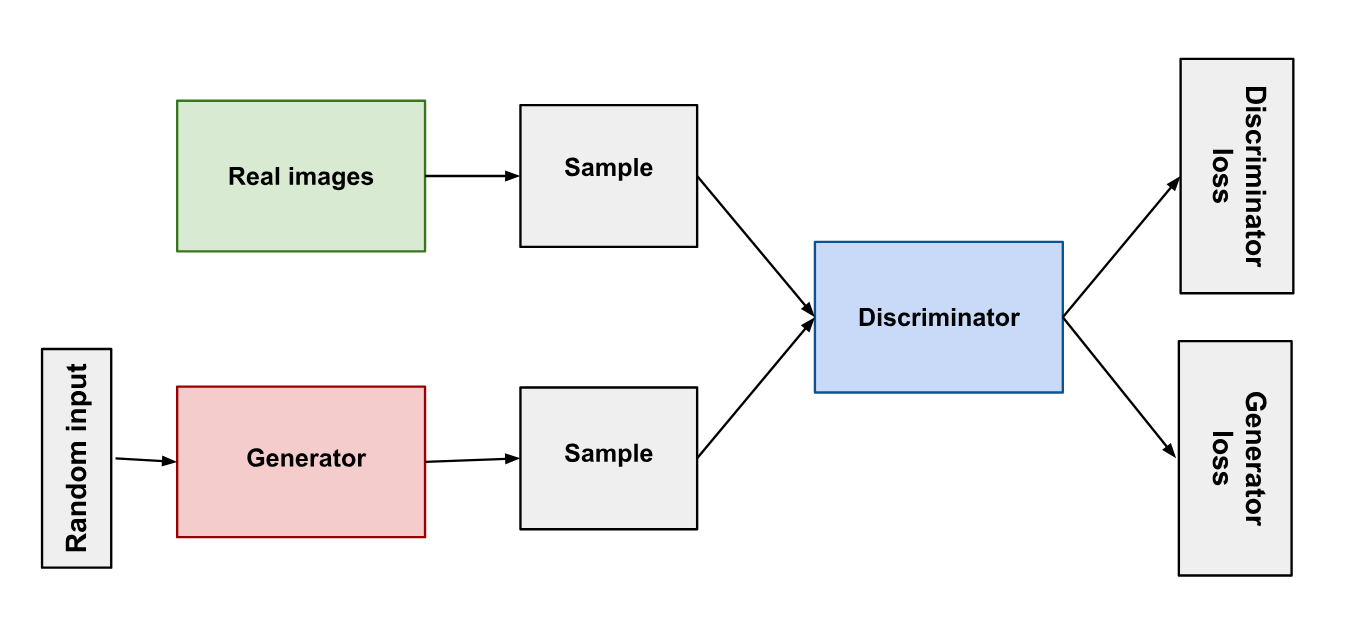
\includegraphics[width=\textwidth]{img/GAN.png}
    \caption{GAN architecture}
\end{figure}

Diffusion models use a different approach to generate images.
\todo[inline]{More on diffusion model}


As improvements happen at an impressive rate in the field of generative models, concerns about security issues rose as well. These tools could be used to manipulate information and combined with social media they would be weapon of massive disinformation. As generative model keep improving, we need to develop new tools to detect generated images. But what should we look for in generated images in order to differentiate them from real images? Many approaches were explored in recent years. Let's go over some of them as they are presented in \autocite*{tariangSyntheticImageVerification2024}.

\subsection{Detection based on high-level artifacts}
These methods detect generated images using a similar approach as humans when they differentiate real and generated images. These approaches look at errors such as incorrect perspectives, incoherence in lighting and shadows or asymmetries in faces.

\subsection{Detection based on low-level artifacts}
AI-generated images contain artifacts in the Fourier domain of the model used to generate them. Detecting these traces is a way to detect whether an image is AI-generated. Many generation models contain an upsampling operation in their generation pipeline. An alternative approach to exploit high-frequency artifacts is to look at the noise residuals by removing the scene content. Nonetheless, these approaches are weak to post processing of images. If for instance, jpeg compression is applied, low-level information can be lost making it impossible to correctly classify an image.
\begin{figure}[H]
    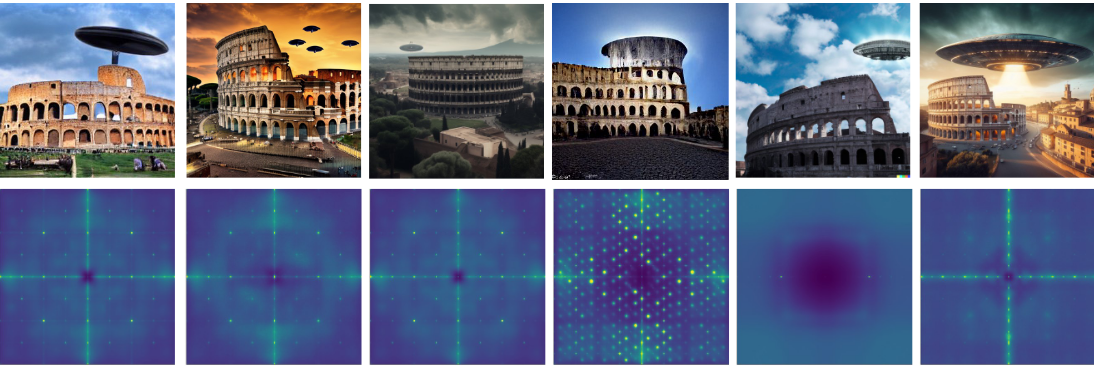
\includegraphics[width=\textwidth]{img/peaks.png}
    \caption{Figure and caption extracted from \autocite*{tariangSyntheticImageVerification2024}. Top: examples of synthetic images, generated using (from left to right) Latent Diffusion, Stable Diffusion, Midjourney v5, DALL·E Mini, DALL·E 2, DALL·E 3. The prompt used for their generation is the following: a photo of the Rome Colosseum with a UFO over it, detailed, 8k. Bottom: Average Power Spectra of the artificial fingerprints for each of such model. Forensic artifacts are clearly visible as spectral peaks in the Fourier domain, stronger or weaker based on the specific model. We can observe that the first three images share very similar artifacts while the fingerprints of the three releases of DALL-E differ greatly from one another, testifying to very different generative architectures.}
\end{figure}

\subsection{Data-driven approaches}
Early method for synthetic image detection were based on CNN architecture with a lot of data. Trying to learn useful features that could help differentiating real and generated images. These first approaches worked well when training and testing data were very similar but had poor generalization capability. To address this robustness issue, researchers used deep CNN architectures combined with augmentation at training time. Augmentations included compressed and blurred images. The diversity of the data used for training also plays a crucial role in a detector's ability to generalize. More recent works delved into architectures different from CNN. In \autocite*{cozzolinoRaisingBarAIgenerated2024}, authors showcased the good performances of CLIP-ViT\footnote{ViT: Vision Transformer} for this type of classification. Within my team, I worked on a semantic approach using CLIP and \autocite*{cozzolinoRaisingBarAIgenerated2024} as a starting point.\\
CLIP (Contrastive Language-Image Pretraining) is a neural networked introduced by OpenAI in \autocite*{radfordLearningTransferableVisual2021}. This network was trained on a massive amount of (text,image) pairs and can then be used with no modification for zero-shot classification. This network training is called contrastive learning. The goal of contrastive learning, as it is stated in \autocite*{tianContrastiveMultiviewCoding2020}, is to learn an embedding that contrasts samples from two distributions. In the case of CLIP, we consider the training dataset to be the following : $\{t_i,\ img_i\}_{i=1}^N$ where $t_i$ is the text associated to the image $img_i$. Each pair contains a textual representation and a visual representation of the same object. We can consider that we thus have a distribution of texts and a distribution of images, which are the marginals, and we have the joint distribution which is the one of the pairs of texts and images. Contrastive learning will separate samles of the joint from sample of the product of marginals. In practice, the model learns to maximize in a latent space the cosine similarity between congruent pairs (e.g.\{"cat", image of a cat\}) and minimize cosine similarity between incongruent pairs (e.g. \{"dog", image of cat\}). As we work in a latent space, it implies that we have encoders to perform the embedding. In the case of CLIP-ViT, transformer-based architectures are used for both the text encoder and the image encoder. Many pretrained versions of CLIP are available online. In our case we used the model proposed by LAION: CLIP ViT-L-14, an open source implementation of CLIP trained on DataComp-1B, a dataset of 1.28B pairs of (text, image) pairs.
\begin{figure}[H]
    \includegraphics*[width=\textwidth]{img/CLIP.png}
    \caption{Figure from \autocite*{radfordLearningTransferableVisual2021}. Images and text are embedded in a latent space, the cosine similarity is then computed on pairs of texts and images.}
\end{figure}


\section{Contributions and associated results}
\subsection{Impact of JPEG compression}
\subsection{Adding diversity to the data}
\subsection{Bigger datasets and neural network}
\subsection{Pair training}
\subsection{Filling the holes with fine tuning}

\subsection{Color features}

\subsection{DINO as an alternative to CLIP}
\autocite*{oquabDINOv2LearningRobust2024}

\subsection{Tip-Adapter}
\autocite*{khanCLIPpingDeceptionAdapting2024}
\autocite*{zhangTipAdapterTrainingfreeAdaption2022}


\section{Conclusion and perspectives}
\subsection{Understanding CLIP features}
AID real img are bad crops with poor semantic content so why does CLIP detector performed well ?
Adversarial attack.

\newpage
\printbibliography

\end{document}